\chapter{Problem Definition}\label{ch:problem-definition}
\section{Introduction}\label{sec:pd-intro}
The system we consider in this thesis is Interactive Myocontrol (section \ref{sec:interactivemyocontrol}), as we have seen in the relative section the input data of our machine learned controller comes from the eight sEMG sensors of the myobracelet and the output data are the activation levels of the nine DOFs of the prosthetic hand.
The problem we are going to study is what we call \textit{activation overshooting}: whenever a participant increase her muscle activation we expect that the prosthesis would in turn increase the applied force / torque; however, if we have a non-linear learning model like the one used in Interactive Myocontrol, this behaviour is not guaranteed. This kind of behaviour should be prevented and avoided by all means because can easily lead to potentially catastrophic failures: in practice whenever a participants increase her force in order to acquire, for example, a better grip on an object the results is the opposite to her expectation, e.g. the prosthesis drop the object.
Overshooting cannot be easily solved gathering more training data for the participant: this would require her to apply a large amount of force which could lead her to muscle strain, fatigue and frustration. Therefore we decided to study in the direction of "mechanically" amend the machine learning model in order to make it more reliable with respect to overshooting.
\section{Formal Definition}
In order to be able to amend the machine using an automated procedure we needed to define the overshooting problem in a strictly formal way: in the following we show how we arrived to the formal definition.
For sake of convenience we briefly consider a 2D-reduced exemplary S in which are contained the samples generated by three actions: rest, power grasp and wrist flexion. As can be seen in figure \ref{fig:heatmap} the training set can be seen as a set of clusters, each corresponding to a certain action.
\begin{figure}[ht]
    \centering
    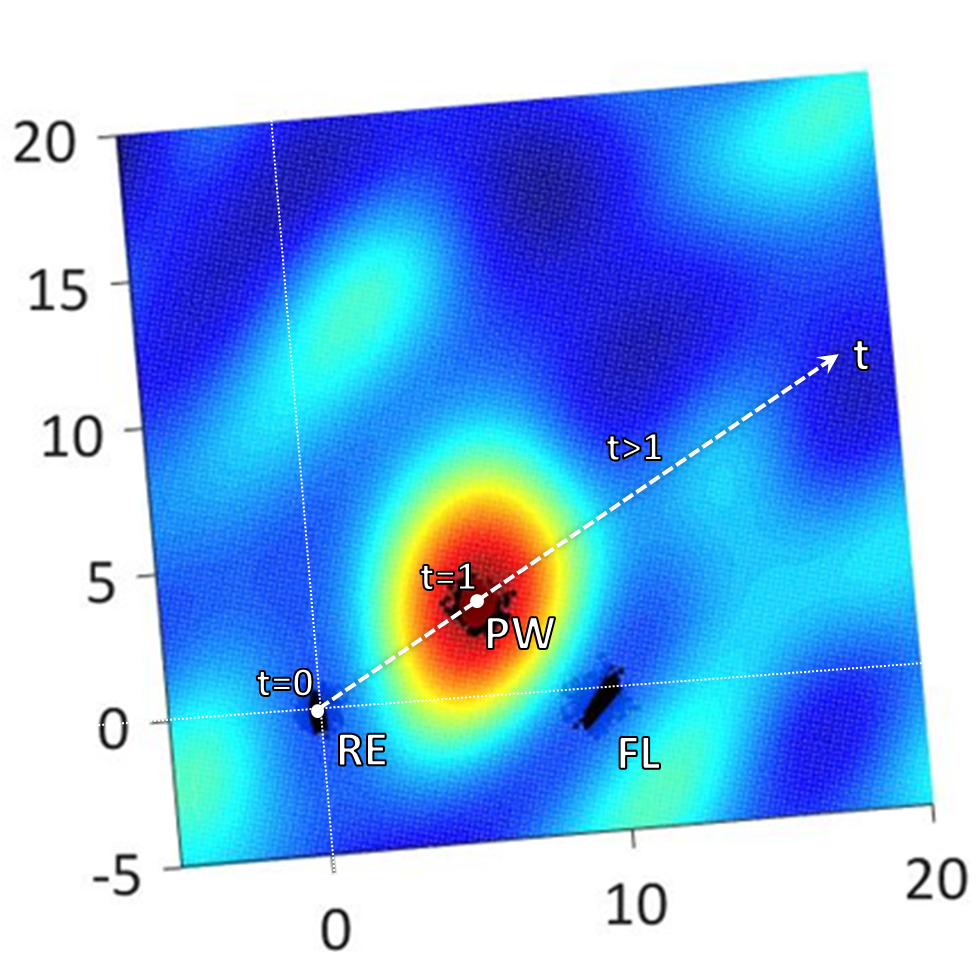
\includegraphics[width=0.8\textwidth]{Images/heatmap_DOF1.png}
    \caption{A 2D-reduced exemplary dataset S, obtained after gathering observations for three actions (black dots; rest, RE; power grasp, PW; wrist flexion, FL); the colour of the heat map denotes the value of the target value for power grasping, $f_{PW}$ . Values of the input space lying on the straight line $\overline{RE} + (\overline{PW} - \overline{RE})t_{PW}$ roughly denote power grasping with increasing strength.}
    \label{fig:heatmap}
\end{figure}
We define as $\overline{RE}$, $\overline{PW}$, $\overline{FL}$ the centers of the clusters corresponding respectively to the actions rest, power grasp and wrist flexion. In the figure is possible to see, as an heatmap, the function $f_{PW}$ obtained by training the learning model seen in section \ref{sec:ML} using the training set S.  
We decided to assume the straight line of the type $\overline{RE} + (\overline{PW} - \overline{RE})t_{PW}$ as the zone of the input space along which the participants signals move when she increase or decrease the force applied to a certain action; this assumption is justified by the physiology of the muscular activation and by our experimental observation.
As can be seen in figure \ref{fig:heatmap} between $t_{PW} = 0$ and $t_{PW} = 1$ the behaviour of the model is what we expected: the value of $f_{PW}$ increase with $t_{PW}$ and assume the maximum value for $t_{PW} = 1$, which corresponds to $\overline{PW}$. The problem become clear for the values of $t_{PW}$ greater than 1: almost immediately $f_{PW}$ begin to decrease and reaches 0 for $t_{PW} \approx 2$. In practice, the participant tries to apply more force and instead the hand open up, leading to drop the grasped object. This kind of failure is what we have called overshooting.
We are now able to give a formal definition of a model subject to overshooting:
\begin{equation}
    \exists a,t_a>1 : x = \overline{RE} + (\overline{a} - \overline{RE})t_{a} \implies f_a(x) < a_{max}
    \label{eq:overshooting}
\end{equation}
where $a$ indicates a general action on which we have trained the model and $a_{max}$ is the maximum activation value for that action. The other quantities correspond to what we have seen before but for a general action $a$.